% Time-stamp: <2015-04-10 17:56:40 chl>

%
% Here is a temptative textbook on R graphics with the lattice package.
%

\documentclass[a4paper,twoside]{book}
\let\newfloat\undefined

% Some packages I need: mdframed (colored frames with rounded corners)
% because using tikz would simply be... too much; graphicx for
% handling images (of course!); url (at some point, I'll need to
% decide whether to rely on href or not); and xspace to handle leading
% space after \R. The lipsum package should be removed when I don't
% need it anymore.
\usepackage[framemethod=1,skipbelow=\topskip,skipabove=\topskip]{mdframed}
\usepackage{graphicx}
\usepackage{url}
\usepackage{lipsum}
\usepackage{xspace}

% Override default headings and chapter style
\usepackage{fancyhdr}
\usepackage[Sonny]{fncychap}
\usepackage[eventxtindent=3pt,oddtxtexdent=3pt]{thumbs}

% Use margin note
\usepackage{marginnote}

% Hmisc Tables
\usepackage{ctable,setspace,relsize}

% To handle illustrated code chunks, I'm using a combination of the
% following two packages:
\usepackage{caption}
\usepackage{subfig}
\usepackage{floatrow}

% \makeatletter\@mparswitchfalse\makeatother
% \DeclareMarginSet{hangleft}%
% {\setfloatmargins
%   {\hskip-\marginparwidth\hskip-\marginparsep}{\hfil}}
% \DeclareColorBox{framedfigure}{\fcolorbox{gray}{white}}

\floatsetup[figure]{facing=yes,capbesideposition={top,inside},capbesidesep=quad}
\floatsetup[widefloat]{margins=hangoutside,
                       %captionskip=3pt,
                       %framestyle=colorbox,framefit=yes,
                       %colorframeset=framedfigure,
                       %frameset={\fboxrule3pt\fboxsep8pt},
                       %framestyle=fbox,framearound=row,
                       %frameset={\fboxrule1pt\fboxsep10pt},
                       style=plaintop}
\captionsetup[widefloat]{justification=RaggedRight,name=Box,skip=15pt,
                         font={sf},labelfont={normalsize,sf,bf},
                         labelsep=newline,strut=no}

% and this is to avoid leaving too much blank between adjacent floats
\setlength{\floatsep}{1.25\baselineskip plus 3pt minus 2pt}
\setlength{\intextsep}{1.2ex}

% Some extra symbols (to mimic R's pch=0,1)
\usepackage{wasysym}

% Here is for the index
\usepackage{makeidx}
\usepackage{multicol}
\makeatletter
\renewenvironment{theindex}
  {\if@twocolumn
      \@restonecolfalse
   \else
      \@restonecoltrue
   \fi
   \setlength{\columnseprule}{0pt}
   \setlength{\columnsep}{35pt}
   \begin{multicols}{3}[\section*{\indexname}]
   \markboth{\MakeUppercase\indexname}%
            {\MakeUppercase\indexname}%
   \thispagestyle{plain}\footnotesize
   \setlength{\parindent}{0pt}
   \setlength{\parskip}{0pt plus 0.3pt}
   \relax
   \let\item\@idxitem}%
  {\end{multicols}\if@restonecol\onecolumn\else\clearpage\fi}
\makeatother

% I'm collecting pictures from a single PDF file generated by R.
% The macro takes one argument, although it should not be necessary
% because I'm using a single PDF file. However, I thought of extending
% this textbook to ggplot, in which case I would need to handle two
% PDF files of external figures.
\usepackage{pdfpages}
\newcounter{fig}
\setcounter{fig}{1}
\newcommand{\img}[1]{\includegraphics[page={\value{fig}},width=2in]{#1}\stepcounter{fig}}
\newcommand{\simg}[1]{\includegraphics[page={\value{fig}},width=1.5in]{#1}\stepcounter{fig}}

% Version control
\immediate\write18{sh ./vc}
%%% This file has been generated by the vc bundle for TeX.
%%% Do not edit this file!
%%%
%%% Define Git specific macros.
\gdef\GITHash{7d26af967a77cf0297c0a8399d8e7d89ee73496d}%
\gdef\GITAbrHash{7d26af9}%
\gdef\GITParentHashes{d83783008f34c984f681d3152721e47e478d7891}%
\gdef\GITAbrParentHashes{d837830}%
\gdef\GITAuthorName{Christophe Lalanne}%
\gdef\GITAuthorEmail{ch.lalanne@gmail.com}%
\gdef\GITAuthorDate{2015-04-10 17:58:32 +0200}%
\gdef\GITCommitterName{Christophe Lalanne}%
\gdef\GITCommitterEmail{ch.lalanne@gmail.com}%
\gdef\GITCommitterDate{2015-04-10 17:58:32 +0200}%
%%% Define generic version control macros.
\gdef\VCRevision{\GITAbrHash}%
\gdef\VCAuthor{\GITAuthorName}%
\gdef\VCDateRAW{2015-04-10}%
\gdef\VCDateISO{2015-04-10}%
\gdef\VCDateTEX{2015/04/10}%
\gdef\VCTime{17:58:32 +0200}%
\gdef\VCModifiedText{\textcolor{red}{with local modifications!}}%
%%% Assume clean working copy.
\gdef\VCModified{0}%
\gdef\VCRevisionMod{\VCRevision}%


% Bibliography management
\usepackage[style=verbose-trad2,natbib=true]{biblatex}
\bibliography{refs}
\usepackage[hang,flushmargin]{footmisc} 

% Setup for XeLaTeX
\usepackage{fontspec,xltxtra,xunicode}
\usepackage{unicode-math}
\defaultfontfeatures{Scale=MatchLowercase}
\setromanfont[Mapping=tex-text]{Minion Pro} 
\setmathfont{Asana Math} 
\setsansfont[Mapping=tex-text]{Myriad Pro} 
\setmonofont[Scale=0.91]{Inconsolata}
\newfontfamily{\titlefont}[Scale=1.4]{Fertigo Pro}

% Some custom colors (not all needed)
\definecolor{grey30}{rgb}{.3,.3,.3}
\definecolor{grey70}{rgb}{.7,.7,.7}
\definecolor{mybrown}{rgb}{.5,.4,.3}
\definecolor{myred}{rgb}{.75,.19,.19}
\definecolor{myred2}{rgb}{.87,.38,.38}
\definecolor{myred3}{rgb}{.65,.38,.38}
\definecolor{myred4}{rgb}{.83,.64,.64}
\definecolor{shadecolor}{rgb}{.87,.93,.89}
\definecolor{cornflowerblue}{rgb}{.39,.58,.93}
\definecolor{seagreen}{rgb}{.18,.54,.34}
\definecolor{dandelion}{rgb}{.94,.88,.19}
\definecolor{peach}{rgb}{.996,.851,.723}
\definecolor{tan}{rgb}{.82,.70,.55}
\definecolor{periwinkle}{rgb}{.80,.80,1}



% Here is how I customized a listings environment for pretty printing
% R code. Keywords are highlighted and automatically appended to the
% index file.
\usepackage[formats]{listings}
\lstdefineformat{tilde}{\~=\textcolor{myred3}{$\mathtt{\sim}$}}
\lstloadlanguages{R} 
\lstdefinelanguage{Renhanced}[]{R}{% 
   morekeywords={data.frame,within,as.numeric,cut,xyplot,histogram,%
                 groups,breaks,include.lowest,with,pch,panel.xyplot,%
                 replicate,alpha,colorRampPalette,jitter.x,amount,%
                 panel.rug,brewer.pal,rgb,jitter.y,describe,%
                 summary.formula,type,scales,xscale.components,%
                 yscale.components,xscale.components.log10.3,%
                 yscale.components.log10.3,box.ratio,limits,at,%
                 panel.bwplot,panel.points,cex,zoo,plot.points,%
                 ref,panel.histogram,panel.mathdensity,dmath,border,%
                 densityplot,nint,tck,alternating,boxplot.stats,%
                 na.rm,span,jitter.data,horizontal,draw,stripchart,%
                 aspect,seg.col,seg.lwd,xlab,ylab,varwidth,fill,bw,%
                 par.settings,simpleTheme,lwd,panel.xyarea,lag,%
                 panel.superpose,superpose,group.number,panel.groups,%
                 overlap,ts.union,layer,panel.tskernel,panel.lines,%
                 rollmean,number,strip,strip.left,filter,panel.xblocks,%
                 method,auto.key,columns,horizonplot,colorkey,qqmath,%
                 ecdfplot,dist,f.value,FUN,barchart,lty,panel.average,%
                 fun,col.regions,rot,scale,relevel,cut2,as.character,%
                 adj,panel.text,bystats,bystats2,summarize,summary.formula,%
                 colMeans,mApply,cut2,as.data.frame,matrix2dataFrame,%
                 impute,transcan,aregImpute,select}, 
   deletekeywords={*,/,gaussian,count}}
\lstset{language=Renhanced,
	format=tilde,
	keepspaces=true,
	%escapeinside={\%*}{*)},
	extendedchars=true, 
	alsoletter={.},
	upquote=true,
	basicstyle=\small\ttfamily, 
   	commentstyle=\color{myred4}, 
   	keywordstyle=\color{myred3}, 
   	showstringspaces=false, 
   	index=[1][keywords], 
   	indexstyle=\indexfoo} 
\newcommand{\indexfoo}[1]{\index{#1@\textcolor{grey30}{\tt #1}}} 
%\lstalias{Rcap}{Renhanced}
\makeatletter
\lst@AddToHook{TextStyle}{\let\lst@basicstyle\normalsize\ttfamily}
\makeatother

% I also redefine verbatim text to be handled by listings. This is
% weird because every verbatim is going to be treated as R code, but
% it is handy at some point. The rest is purely to avoid typing the
% same text repetitively.
\renewcommand{\texttt}[1]{\lstinline{#1}}
%\makeatletter
%\lst@AddToHook{Rcap}{\let\lst@basicstyle\small}
%\makeatother
\newcommand{\R}{\textsf{R}\xspace}
\newcommand{\mytilde}{\textcolor{myred3}{$\sim$}\xspace}

% R code chunk are embedded in a smooth color frame. (That's also
% weird because I cannot use lstlistings for any other purpose, whih
% is why I'll be using standard verbatim environment for R session or
% other stuff.)
\mdfsetup{innerbottommargin=0pt,leftmargin=0pt,rightmargin=0pt,%
          backgroundcolor=shadecolor,linecolor=none,roundcorner=5}
\BeforeBeginEnvironment{lstlisting}{\begin{mdframed}\vskip-.5\baselineskip}
\AfterEndEnvironment{lstlisting}{\end{mdframed}}

% I'm using temporarily this example title page, roughly copy/pasted from the 
% Memoir class package.
\definecolor{Medium}{gray}{.6}
\newlength{\tpheight}\setlength{\tpheight}{0.9\textheight}
\newlength{\txtheight}\setlength{\txtheight}{0.9\tpheight}
\renewcommand*{\marginfont}{\color{grey70}\sffamily\footnotesize}

% I don't want indentation for new paragraph, but just increase
% vertical separation between them.
\setlength{\parindent}{0pt}
\setlength{\parskip}{1ex plus 0.5ex minus 0.2ex}

% That's the magic command to tell LaTeX to start indexing the document.
\makeindex

%
% End of preamble.
%

\begin{document}
\pagenumbering{arabic}
\pagestyle{empty}

% This is merely a copy/paste from the memoir class, see T&H
% Typography.
% I should rework it when I have time, though I find it pretty nice
% actually...
\begingroup% 
\raggedleft
\vspace*{\baselineskip}
{\Large\textsf{Christophe Lalanne}}\\[0.167\txtheight]
{\Large\titlefont A Visual Guide to}\\[\baselineskip]
{\textcolor{Medium}{\Huge\titlefont R Graphics and}}\\[\baselineskip]
{\textcolor{Medium}{\Huge\titlefont Data Munging}}\\[\baselineskip]
{\tiny\titlefont With 65 illustrations}\par
\vfill
{
\includegraphics[scale=.75]{logo}\\{\small \tt \GITAbrHash}\\{\small
    \tt \VCDateTEX}}\par 
\vspace*{3\baselineskip}
\endgroup
\pagestyle{empty}
\cleardoublepage

\frontmatter
\pagestyle{empty}
\vspace*{\fill}
\centerline{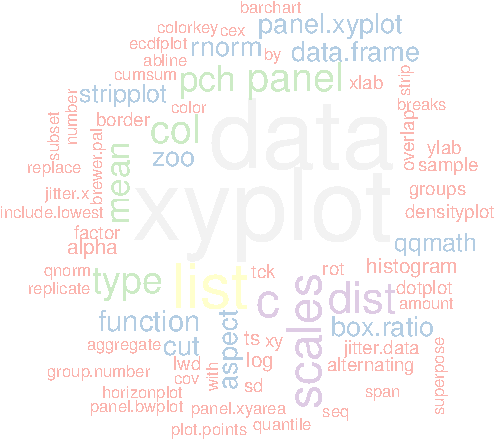
\includegraphics[width=.6\textwidth]{wcindex}}
\vspace*{3\baselineskip}
\hfill{\footnotesize \emph{The greatest value of a picture is when it forces us to notice what we
never expected to see}. --- John Tukey}

\hfill{\footnotesize \emph{At their best, graphics are instruments for reasoning}. --- Edward Tufte}
\vspace*{\fill}
\cleardoublepage
\pagenumbering{roman}
\tableofcontents

\mainmatter
\pagenumbering{arabic}
% --------------------------------------------------------------- Chapter 1 --
\chapter{Getting started with \R graphics}

\section{Why \R?}
In the ``GNU world'', most of the plotting program expect data from
text file (tab-delimited or csv) arranged by columns, with extra
grouping levels denoted by string or integer codes. This is the case
with \textsf{gnuplot}\autocite{janert09} (\url{http://www.gnuplot.info/}) or
\textsf{plotutils} (\url{http://www.gnu.org/software/plotutils/}), for
example. 

Here is how we could create an histogram in gnuplot, from a series of
500 gaussian variates generate using \R as follows:
\begin{verbatim}
$ Rscript -e 'cat(rnorm(500), sep="\\n")' > rnd.dat
\end{verbatim}

Then, in gnuplot, we can run
\begin{verbatim}
bw=0.2
n=500
bin(x,width)=width*int(x/width)
tstr(n)=sprintf("Binwidth = %1.1f\n", n)
set xrange [-3:3]
set yrange [0:1]
set boxwidth bw
plot 'rnd.dat' using (bin($1,bw)):(1./(bw*n)) smooth frequency \
  with boxes title tstr(bw)
\end{verbatim}

to get the picture shown below. (Note that we didn't try to customize
anything, except the title.)

\centerline{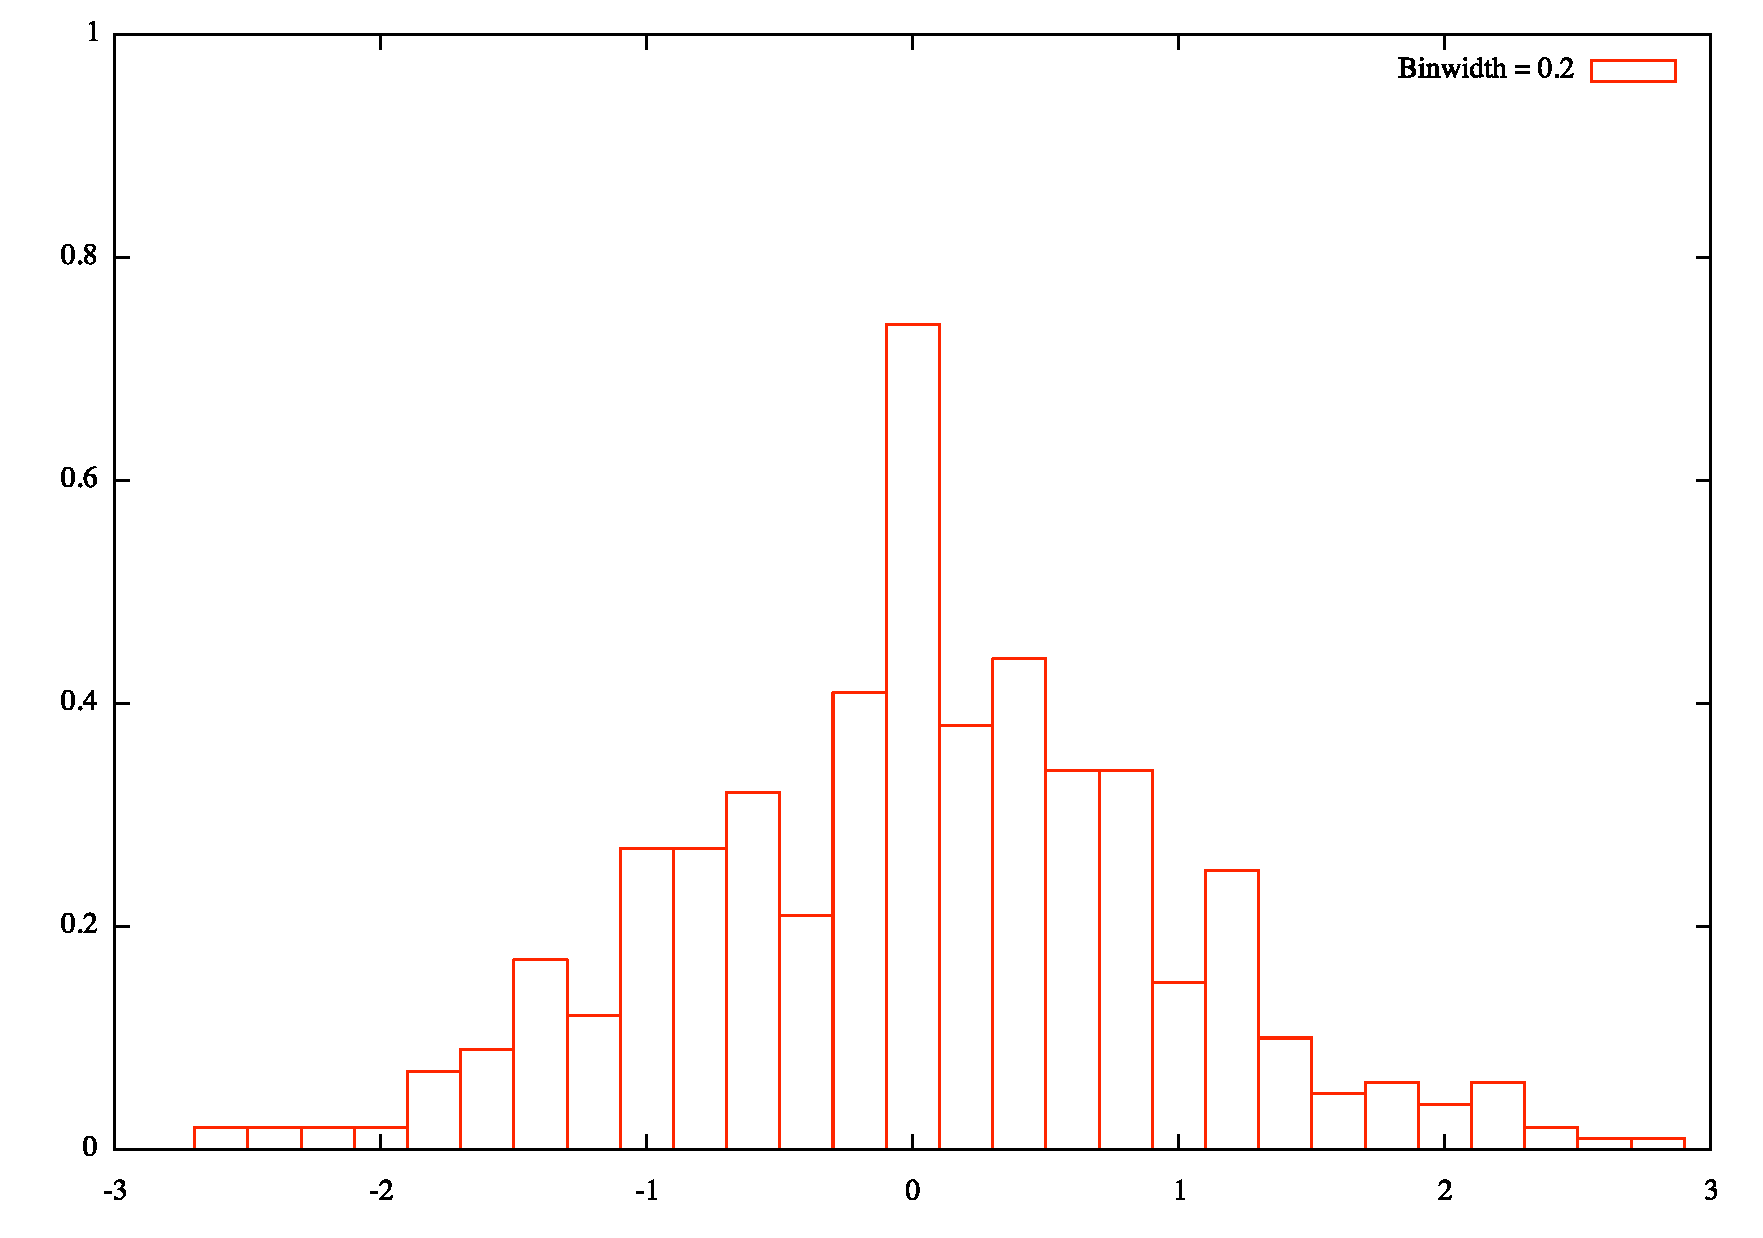
\includegraphics[width=.75\textwidth]{gnuplot}}

The above example shows one important aspect of using a dedicated
statistical package: \textsf{Gnuplot} has no function to draw an
histogram, and we have to write some code to perform additional tasks,
like binning in this case. The same applies for
\textsf{plotutils}. We could make use of external programs to do that,
like the \textsf{GSL} library (see example~22.11 from the manual,
\url{http://www.gnu.org/software/gsl/manual/}), but this two-stage
approach is rather likely to be cumbersome for repetitive tasks.

The author found that \textsf{Stata} is one of the only great
alternative to \R, but it has its cost. In fact, this textbook is
largely inspired from one of Stata Press book on \textsf{Stata}
graphical capabilities\autocite{mitchell08}.

\section{The \R graphical model}

\section{Base vs. {\tt lattice} graphics}

\section{The grammar of graphics}

% --------------------------------------------------------------- Chapter 2 --
\chapter{Data management}
\addthumb{Data munging}{\Large\textsf{Tidying}}{white}{cornflowerblue}

\section{Structuring data}
In R, the most common structure used to store a data set with
mixed-type variables is a \texttt{data.frame}. Such an \R object
presents several characteristics that makes it most appropriate for
managing statistical data structure, with few exceptions (e.g., when
one only has to work with aggregated data or two-way tables). It
should be noted that other data structures might be more appropriate,
for example when one is interested in time series analysis, but see
the \texttt{zoo} package\autocite{zeilis05}.

Many \R functions accept \texttt{data.frame} as input, and further
allow to subset or index it for computation or visualization
purpose. In addition to receiving a \texttt{data.frame}, some \R
commands allow to use a \emph{formula} notation, where the right and
left-hand side are separated by the \mytilde (tilde) operator. The
use of \index{formula} together with a \texttt{data.frame} simplify the
accession of variable in a given environment.
This is especially true when using the \texttt{lattice} package which
is entirely based on formula, even if this is not apparent at
first sight.

\section{Managing data}
Consider, for example, the \emph{low birth study} which is discussed
at length in Hosmer and Lemeshow's textbook on logistic regression
\autocite{hosmer89}. A quick look at the variables should make it
clear that they won't be treated the way we like them to be
considered: mother's ethnicity status (\texttt{race}) takes three
integer values, without any explicit meaning.

\begin{verbatim}
data(birthwt, package="MASS")
str(birthwt)
\end{verbatim}

\subsection{Variable recoding and annotation}
The \texttt{Hmisc} package includes numerous \R functions that will
facilitate the task of data checking (\texttt{describe} provides
``codebook'' facilities), summarizing (\texttt{summary.formula}) or
aggregating data, (\texttt{summary.formula}).

Here are some examples of use with the \texttt{birthwt} data. For
illustration purpose, we set some observations as missing on two variables
(\texttt{age} and \texttt{ftv}).

\begin{verbatim}
set.seed(101)
birthwt$age[5] <- NA
birthwt$ftv[sample(1:nrow(birthwt), 5)] <- NA
yesno <- c("No", "Yes")
birthwt <- within(birthwt, {
    smoke <- factor(smoke, labels = yesno)
    low <- factor(low, labels = yesno)
    ht <- factor(ht, labels = yesno)
    ui <- factor(ui, labels = yesno)
    race <- factor(race, levels = 1:3, labels = c("White", "Black", "Other"))
    lwt <- lwt/2.2  ## weight in kg
})
\end{verbatim}

It often helps to keep variable names short and informative, and to have
separated labels and/or units in case of continuous measurements. This is
available via the \texttt{label} and \texttt{units} functions. Note that
\texttt{label} allows to annotate the data frame as well.

\begin{verbatim}
library(Hmisc)
label(birthwt$age) <- "Mother age"
units(birthwt$age) <- "years"
label(birthwt$bwt) <- "Baby weight"
units(birthwt$bwt) <- "grams"
label(birthwt, self = TRUE) <- "Hosmer & Lemeshow's low birth weight study."
\end{verbatim}

These labels can then be used in almost every \texttt{Hmisc} functions, even
when using \texttt{list.tree} in place of \texttt{str}. However, we will see
that there mostly useful when generating Tables or Figures.

The \texttt{contents} command offers a quick summary of data format and
missing values, and it provides a list of labels associated to variables
treated as factor by R.

Once we have a working data frame, the functions \texttt{contents} and
\texttt{describe} provide two quick summary of the data.

\begin{verbatim}
> contents(birthwt)

Data frame:birthwt	189 observations and 10 variables    Maximum # NAs:5


           Labels Units Levels   Class Storage NAs
low                          2         integer   0
age    Mother age years        integer integer   1
lwt                                     double   0
race                         3         integer   0
smoke                        2         integer   0
ptl                                    integer   0
ht                           2         integer   0
ui                           2         integer   0
ftv                                    integer   5
bwt   Baby weight grams        integer integer   0

+--------+-----------------+
|Variable|Levels           |
+--------+-----------------+
|  low   |No,Yes           |
|  smoke |                 |
|  ht    |                 |
|  ui    |                 |
+--------+-----------------+
|  race  |White,Black,Other|
+--------+-----------------+
\end{verbatim}

As can be seen, \texttt{contents} displays storage mode and class of R
variables that are present in the data frame. The number of missing values
is also reported for each variable. The levels of each \texttt{factor}-type
variable is also printed at the end of the output.

\begin{verbatim}
> describe(subset(birthwt, select = c(low, age, race, ftv)), digits = 3)

 4  Variables      189  Observations
--------------------------------------------------------------------------------
low
      n missing  unique
    189       0       2

No (130, 69%), Yes (59, 31%)
--------------------------------------------------------------------------------
age : Mother age [years]
      n missing  unique    Info    Mean     .05     .10     .25     .50     .75
    188       1      24       1    23.3      16      17      19      23      26
    .90     .95
     31      32

lowest : 14 15 16 17 18, highest: 33 34 35 36 45
--------------------------------------------------------------------------------
race
      n missing  unique
    189       0       3

White (96, 51%), Black (26, 14%), Other (67, 35%)
--------------------------------------------------------------------------------
ftv
      n missing  unique    Info    Mean
    184       5       6    0.83   0.783

           0  1  2 3 4 6
Frequency 98 45 30 7 3 1
%         53 24 16 4 2 1
--------------------------------------------------------------------------------
\end{verbatim}

The \texttt{describe} function gives more details, and, in particular,
provides useful summary statistics for each variable. Here, we only
considered four variables: a binary variable (\texttt{low}), a continuous
measure (\texttt{age}), a three-level factor (\texttt{race}), and a count
variable (\texttt{ftv}). The output will be different depending on the type
of variable, and for all but continuous measures (defined as variable taking
at least 10 distinct values) \texttt{describe} will display a table of
counts and frequencies.

\subsection{Variable transformation}
In case we would like to consider one of the above factors as a
numerical variable, we can now use \texttt{as.numeric} and \R will
take care of attributing the lowest integer score to the baseline
category. Of course, there might be occasion where we would like to
change that reference level; or, we might want to collapse two
discrete categories. Again, there are simple commands to do that, for
example:
\begin{verbatim}
birthwt$low <- relevel(birthwt$low, "Yes")
levels(birthwt$race)[2:3] <- "Black+Other"
\end{verbatim}

Another common task consists in transforming some predictors, either
for visualization purpose or when building an explantory or predictive
model. As a simple example, we can imagine centering some of the
predictors of interest, like \texttt{age}, in the above example. The
\texttt{within} or \texttt{transform} command can be used to append
the centered variable to the list of variables present in the
\texttt{data.frame}:
\begin{verbatim}
birthwt <- transform(birthwt, age.c=scale(age, scale=FALSE))
\end{verbatim}

Likewise, we may want to recode previous premature labours
(\texttt{ptl}) as yes/no and number of physician visits during the
first trimester (\texttt{ftv}) as one/more than one, like shown below
(we show two different syntax that basically perform the same task by
relying on \R indexing):
\begin{verbatim}
birthwt <- transform(birthwt, ptl.yn=factor(ptl > 0, labels=c("No","Yes")), 
                     ftv.c=factor(ifelse(ftv < 2, "1", "2+")))
\end{verbatim}

\texttt{Hmisc} provides a replacement for R's \texttt{cut} function with
better default options (especially the infamous \texttt{include.lowest =
  FALSE}) to discretize a continuous variable. The \texttt{cut2} function
has many useful options, including \texttt{g=} and \texttt{levels.mean=} to
return $g$ classes and report center of each class instead of class
intervals:
\begin{verbatim}
table(cut2(birthwt$age, g = 3, levels.mean = TRUE, digits = 3))
\end{verbatim}

If there is some reason to treat \texttt{ftv} as an ordered factor,
a command like
\begin{verbatim}
as.ordered(cut2(birthwt$ftv, c(0, 1, 2, 6)))
\end{verbatim}
might do the job.

\section{Indexing, subsetting, conditioning}
A lot of statistical operations that practictioners use to apply on a
given dataset are mostly variations around the idea of indexing or
subsetting. By comparison, SQL-like operations would be selection and
projection. 

% FIXME: add more details here

The \texttt{subset} command offers a simple and elegant way to combine both
operations: for a given data frame, the \texttt{subset =} option is used to
filter rows according to logical expression or simple row indexes while the
\texttt{select =} option is used to return only selected variables based on
their index (e.g., column 1 and 3) or an unquoted name (e.g.,
\texttt{c(low,lwt)}). 

The following instruction will print the age of hypertensive mothers whose
baby was underweight:
\begin{verbatim}
subset(birthwt, low == "Yes" & ht == "Yes", age)
\end{verbatim}
It should be noted that \texttt{subset} returns a data frame.

Some people might prefer to use their favorite SQL-like language, so
something like this would perfectly fit their needs:
\begin{verbatim}
library(sqldf)
sqldf("SELECT age FROM birthwt WHERE low = 0 AND ht = 1 LIMIT 3", row.names = TRUE)
\end{verbatim}

Unfortunately, this doesn't work with ``labelled'' objects, as typically
returned by \texttt{Hmisc}, although a solution is readily available at \url{http://stackoverflow.com/q/2394902/420055}.

% FIXME: should be moved in a dedicated subsection?
There are also a bunch of command dedicated to variables clustering,
analysis of missing patterns, or simple (\texttt{impute}) or multiple
(\texttt{aregImpute}, \texttt{transcan}) imputation methods. Here is how we
would impute missing values with the median in the case of a continuous
variable:
\begin{verbatim}
lwt <- birthwt$lwt
lwt[sample(length(lwt), 10)] <- NA
lwt.i <- impute(lwt)
summary(lwt.i)
\end{verbatim}

Missing observations will be marked with an asterisk when we print the whole
object in R. To use the mean instead of the median, we just have to add the
\texttt{fun = mean} option.

\section{Summarizing data}
Statisticians generally spend a great part of their time in data
cleansing, data transformation or re-expression\autocite{hoaglin83},
and data visualization. 

\subsection{Base R functions}
Both the \texttt{by} and \texttt{tapply} function allow to apply a builtin
or custom function to help summarizing a numeric variable by a categorical
variable. Most of the time, these two functions are less handy than
\texttt{aggregate} since the latter offers a formula interface and returns a
data frame. 

\begin{verbatim}
aggregate(bwt ~ ui + I(ftv > 1), data = birthwt, mean)
\end{verbatim}

There is, however, one caveat when using \texttt{aggregate}: even if you can pass a
custom function that returns multiple values that can be printed on screen,
the resulting data frame will still have only one column for its output. For
exemple, the dimensions of the data frame created by the following call to
\texttt{aggregate} is 4 by 3, even if it looks like there two separate
columns for \texttt{bwt} mean and SD.

\begin{verbatim}
f <- function(x) c(mean = mean(x), sd = sd(x))
aggregate(bwt ~ ui + I(ftv > 1), data = birthwt, f)
\end{verbatim}


\subsection{The \texttt{Hmisc} package}

There are three useful commands that provide summary statistics for a list
of variables. They implement the ``split-apply-combine''
strategy\autocite{wickham11} in the spirit of R's built-in functions (unlike
\texttt{plyr}). 

The first one, \texttt{summarize}, can be seen as an equivalent to R's
\texttt{aggregate} command. Given a response variable and one or more
classification factors, it applies a specific function to all data chunk,
where each chunk is defined based on factor levels. The results are stored
in a matrix, which can easily be coerced to a data frame
using, e.g., \texttt{as.data.frame} or \texttt{Hmisc::matrix2dataFrame}. 

Note that enhanced results can be printed on the console using the
\texttt{prn} command. 

Here is a first example, using a dedicated function to print the mean and
standard deviation (SD) of a numerical variable:
\begin{verbatim}
f <- function(x, na.opts = TRUE) c(mean = mean(x, na.rm = na.opts), sd = sd(x, 
    na.rm = na.opts))
out <- with(birthwt, summarize(bwt, race, f))
\end{verbatim}

Here is the output produced by R:
\begin{verbatim}
Average baby weight by ethnicity   out

   race  bwt    sd
3 White 3103 727.9
1 Black 2720 638.7
2 Other 2805 722.2
\end{verbatim}

Contrary to \texttt{aggregate}, this command provides multiway data
structure in case we ask to compute more than one quantity. In this case,
the dimension of \texttt{out} is a 3 by 3 data frame.

Summarizing multivariate responses or predictors is also possible, with either \texttt{summarize} or \texttt{mApply}. Of course, any built-in functions, such as \texttt{colMeans} could be used in place of our custom summary command.

\begin{verbatim}
with(birthwt, summarize(bwt, llist(race, smoke), f))
\end{verbatim}

The second command, \texttt{bystats}, (or \texttt{bystats2} for two-way
tabular output) allows to describe with any custom or built-in function one
or multiple outcome by two explanatory variables, or even more. Sample size
and the number of missing values are also printed. 

With the following instruction,
\begin{verbatim}
with(birthwt, bystats(cbind(bwt, lwt), smoke, race))
\end{verbatim}
we would get
\begin{verbatim}
 Mean of cbind(bwt, lwt) by smoke 

            N  bwt   lwt
No White   44 3429 63.11
Yes White  52 2827 57.41
No Black   16 2854 67.93
Yes Black  10 2504 64.82
No Other   55 2816 54.16
Yes Other  12 2757 56.36
ALL       189 2945 59.01
\end{verbatim}
whereas
\begin{verbatim}
with(birthwt, bystats2(lwt, smoke, race))
\end{verbatim}
gives
\begin{verbatim}
 Mean of lwt by smoke 

+----+
|N   |
|Mean|
+----+
+---+-----+-----+-----+-----+
|No | 44  | 16  | 55  |115  |
|   |63.11|67.93|54.16|59.50|
+---+-----+-----+-----+-----+
|Yes| 52  | 10  | 12  | 74  |
|   |57.41|64.82|56.36|58.24|
+---+-----+-----+-----+-----+
|ALL| 96  | 26  | 67  |189  |
|   |60.02|66.73|54.55|59.01|
+---+-----+-----+-----+-----+
\end{verbatim}

The third and last command is \texttt{summary.formula}, which can be
abbreviated as \texttt{summary} as long as formula is used to describe
variables relationships. There are three main configurations
(\texttt{method=}): "response", where a numerical variable is summarized for
each level of one or more variables (numerical variables will be discretized
in 4 classes), as \texttt{summarize} does; "cross", to compute conditional
and marginal means of several response variables described by at most 3
explanatory variables (again, continuous predictors are represented as
quartiles); "reverse", to summarize univariate distribution of a set of
variables for each level of a classification variable (which appears on the
left-hand side of the formula). Variables are viewed as continuous as long
as they have more than 10 distinct values, but this can be changed by
setting, e.g., \texttt{continuous = 5}. When \texttt{method = "reverse"}, it
is possible to add \texttt{overall = TRUE}, \texttt{test = TRUE} to add
overall statistics and corresponding statistical tests of null effect
between the groups.

Here are some examples of use, with their outputs.

\begin{verbatim}
> summary(bwt ~ race + ht + lwt, data = birthwt)

Baby weight    N=189

+-------+------------+---+----+
|       |            |N  |bwt |
+-------+------------+---+----+
|race   |White       | 96|3103|
|       |Black       | 26|2720|
|       |Other       | 67|2805|
+-------+------------+---+----+
|ht     |No          |177|2972|
|       |Yes         | 12|2537|
+-------+------------+---+----+
|lwt    |[36.4, 50.9)| 53|2656|
|       |[50.9, 55.5)| 43|3059|
|       |[55.5, 64.1)| 46|3075|
|       |[64.1,113.6]| 47|3038|
+-------+------------+---+----+
|Overall|            |189|2945|
+-------+------------+---+----+
\end{verbatim}

\begin{verbatim}
> summary(cbind(lwt, age) ~ race + bwt, data = birthwt, method = "cross")

 mean by race, bwt 

+-------+
|N      |
|Missing|
|lwt    |
|age    |
+-------+
+-----+-----------+-----------+-----------+-----------+-----+
| race|[ 709,2424)|[2424,3005)|[3005,3544)|[3544,4990]| ALL |
+-----+-----------+-----------+-----------+-----------+-----+
|White|    19     |    23     |    20     |    33     | 95  |
|     |   0       |   1       |   0       |   0       |1    |
|     |   55.55   |   57.67   |   62.23   |   63.25   |60.14|
|     |   22.74   |   24.78   |   24.50   |   24.91   |24.36|
+-----+-----------+-----------+-----------+-----------+-----+
|Black|     9     |     9     |     6     |     2     | 26  |
|     |   0       |   0       |   0       |   0       |0    |
|     |   65.10   |   59.70   |   70.83   |   93.41   |66.73|
|     |   23.44   |   20.89   |   20.00   |   20.50   |21.54|
+-----+-----------+-----------+-----------+-----------+-----+
|Other|    20     |    16     |    19     |    12     | 67  |
|     |   0       |   0       |   0       |   0       |0    |
|     |   51.23   |   52.95   |   58.90   |   55.34   |54.55|
|     |   22.20   |   22.69   |   22.26   |   22.50   |22.39|
+-----+-----------+-----------+-----------+-----------+-----+
|ALL  |    48     |    48     |    45     |    47     |188  |
|     |   0       |   1       |   0       |   0       |1    |
|     |   55.54   |   56.48   |   61.97   |   62.51   |59.06|
|     |   22.65   |   23.35   |   22.96   |   24.11   |23.27|
+-----+-----------+-----------+-----------+-----------+-----+
\end{verbatim}

\begin{verbatim}
> summary(low ~ race + ht, data = birthwt, fun = table)

low    N=189

+-------+-----+---+---+---+
|       |     |N  |No |Yes|
+-------+-----+---+---+---+
|race   |White| 96| 73|23 |
|       |Black| 26| 15|11 |
|       |Other| 67| 42|25 |
+-------+-----+---+---+---+
|ht     |No   |177|125|52 |
|       |Yes  | 12|  5| 7 |
+-------+-----+---+---+---+
|Overall|     |189|130|59 |
+-------+-----+---+---+---+
\end{verbatim}

Finally, here is a more complex Table produced by \texttt{summary.formula}
with \texttt{method = "reverse"}.

\begin{verbatim}
out <- summary(low ~ race + age + ui, data = birthwt, method = "reverse", overall = TRUE, 
    test = TRUE)
print(out, prmsd = TRUE, digits = 2)
\end{verbatim}

Although we display the output on the console directly, it is also possible
to build a $\LaTeX$ Table using the \texttt{latex} function.

\begin{verbatim}
latex(out, file = "tab-summary.tex", ctable = TRUE, digits = 1, exclude1 = FALSE, caption = NULL)
\end{verbatim}

Here is the final output

%latex.default(cstats, title = title, caption = caption, rowlabel = rowlabel,     col.just = col.just, numeric.dollar = FALSE, insert.bottom = legend,     rowname = lab, dcolumn = dcolumn, extracolheads = extracolheads,     extracolsize = Nsize, ...)%
\ctable[pos=!tbp,]{lrcccc}{\tnote[]{\noindent {\scriptsize $a$\ }{$b$\ }{\scriptsize $c$\ } represent the lower quartile $a$, the median $b$, and the upper quartile $c$\ for continuous variables.}\tnote[]{$N$\ is the number of non--missing values.}\tnote[]{Numbers after percents are frequencies.}\tnote[]{\indent Tests used:}\tnote[]{\textsuperscript{\normalfont 1}Pearson test; \textsuperscript{\normalfont 2}Wilcoxon test}}{\FL
\multicolumn{1}{l}{}&\multicolumn{1}{c}{N}&\multicolumn{1}{c}{No}&\multicolumn{1}{c}{Yes}&\multicolumn{1}{c}{Combined}&\multicolumn{1}{c}{Test Statistic}\NN
&&\multicolumn{1}{c}{{\scriptsize $N=130$}}&\multicolumn{1}{c}{{\scriptsize $N=59$}}&\multicolumn{1}{c}{{\scriptsize $N=189$}}&\ML
race~:~White&189&56\%~{\scriptsize~(73)}&39\%~{\scriptsize~(23)}&51\%~{\scriptsize~(96)}&$ \chi^{2}_{2}=5 ,~ P=0.08 ^{1} $\NN
~~~~Black&&12\%~{\scriptsize~(15)}&19\%~{\scriptsize~(11)}&14\%~{\scriptsize~(26)}&\NN
~~~~Other&&32\%~{\scriptsize~(42)}&42\%~{\scriptsize~(25)}&35\%~{\scriptsize~(67)}&\NN
Mother~age~\hfill\tiny{years}&188&{\scriptsize 19~}{23 }{\scriptsize 28} &{\scriptsize 20~}{22 }{\scriptsize 25} &{\scriptsize 19~}{23 }{\scriptsize 26} &$ F_{1,186}=1 ,~ P=0.2 ^{2} $\NN
ui~:~No&189&89\%~{\scriptsize~(116)}&76\%~{\scriptsize~(~45)}&85\%~{\scriptsize~(161)}&$ \chi^{2}_{1}=5 ,~ P=0.02 ^{1} $\NN
~~~~Yes&&11\%~{\scriptsize~(~14)}&24\%~{\scriptsize~(~14)}&15\%~{\scriptsize~(~28)}&\LL
}


\subsection{The \texttt{plyr} package}
The \texttt{plyr} package\autocite{wickham11} offers a general
solution to those kind of tasks.

% --------------------------------------------------------------- Chapter 3 --
\chapter{Univariate distributions}
\addthumb{Lattice graphics}{\Large\textsf{Lattice}}{white}{seagreen}

\lipsum[1]

\section{Stripchart}
Stripchart aims at showing the distribution of a series of continuous
measurements (much like scatterplot for 2D data discussed in
\S~\ref{sec:scatterplot}). They are useful for small to moderate
dataset. With large $N$ it is proably better to switch to alternative
displays, see next sections.

\begin{figure}[H]
\begin{lstlisting}
x <- sample(1:30, 25, replace=TRUE)
stripplot(~ x, jitter.data=TRUE, factor=.8, aspect=.5)
\end{lstlisting}
  \fcapside[\FBwidth] {\img{figs_lattice-crop}}
  {\caption*{With this synthetic dataset where several observations
      can take the same value, jittering point locations on the
      horizontal and vertical axes ensures a better representation.}}
\end{figure}

\begin{figure}[H]
\begin{lstlisting}
stripplot(~ x, jitter.data=TRUE, factor=.8, aspect="xy")
\end{lstlisting}
  \fcapside[\FBwidth] {\img{figs_lattice-crop}}
  {\caption*{A better way of flattening the display is to use an
      ``\texttt{xy}'' aspect.}}
\end{figure}

\begin{figure}[H]
\begin{lstlisting}
stripplot(x ~ 1, horizontal=FALSE, jitter.data=TRUE, aspect=1.2,
          scales=list(x=list(draw=F)), xlab="", pch=15, alpha=.5)
\end{lstlisting}
  \fcapside[\FBwidth] {\img{figs_lattice-crop}}
  {\caption*{This is basically the same picture but the $x$ and $y$
      axis have been transposed. We used a different symbol and
      transparency to highlight where replication occurs in the
      data. Obviously, that won't work so nicely with larger sample
      size or a higher density of replication.}}
\end{figure}

\begin{figure}[H]
\begin{lstlisting}
stripplot(~ x, panel=HH::panel.dotplot.tb, cex=1.2, factor=.2)
\end{lstlisting}
  \fcapside[\FBwidth] {\img{figs_lattice-crop}} {\caption*{In contrast
      to the base \texttt{stripchart} function, there is no way of
      imposing a stacked display in \texttt{lattice}. However, there
      is some convenient panel function in the \texttt{HH} package.}}
\end{figure}

\begin{figure}[H]
\begin{lstlisting}
x <- sample(seq(1, 60, by=2), 75, replace=TRUE)
stripplot(1 ~ x, panel=panel.sunflowerplot, col="black", 
          seg.col="black", seg.lwd=1, size=.08)
\end{lstlisting}
  \fcapside[\FBwidth] {\img{figs_lattice-crop}} {\caption*{With
      possible replicates, it is also interesting to use
      ``sunflowers'' where multiple leaves are used for each
      duplicate. The custom panel function mimics the base
      \texttt{sunflowerplot} function. For an alternative way of
      embedding ``sunflowers'' into a \texttt{lattice} display, see
      the following thread on R-help: \url{http://bit.ly/Ig4RTq}. Note
      that we remove $y$-axis annotation using commands presented
      before (i.e., using \texttt{scales=}).}}
\end{figure}

\section{Histograms}
\lipsum[1]

\begin{figure}[H]
\begin{lstlisting}
histogram(~ waiting, data=faithful)
\end{lstlisting}
  \fcapside[\FBwidth] {\img{figs_lattice-crop}}
  {\caption*{\marginnote{\textbf{faithful}. Waiting time between
        eruptions and the duration of the eruption for the Old
        Faithful geyser in Yellowstone National Park, Wyoming, USA.}A
      simple histogram of waiting time expressed as density. Note that
      forgetting the \mytilde operator will raise an error message.}}
\end{figure}

Box~\ref{box:histogram} shows some custom settings with the
\texttt{faithful} dataset.
\lipsum[1]

\begin{figure*}[h]\fboxsep-.4pt
\ffigbox{}{\CommonHeightRow{\begin{subfloatrow}[4]
\ffigbox[\FBwidth]
{\simg{figs_lattice-crop}}{\caption*{\texttt{type="count"}}}
\ffigbox[\FBwidth]
{\simg{figs_lattice-crop}}{\caption*{\texttt{col="steelblue"}}}
\ffigbox[\FBwidth]
{\simg{figs_lattice-crop}}{\caption*{\texttt{border=NA,
      nint=12}}}
\ffigbox[\FBwidth]
{\simg{figs_lattice-crop}}{\caption*{\texttt{nint=nrow(dataset)}}}
\end{subfloatrow}}
{\caption{Common options for \texttt{histogram} include displaying
    counts instead of percents, or varying bar color. It is also
    possible to change default bin size. When
    \texttt{nint=nrow(dataset)}, we have a so-called high-density
    vertical lines, much like when using \texttt{plot(...,
      type="h")}.}\label{box:histogram}}} 
\end{figure*}


\begin{figure}[H]
\begin{lstlisting}
p <- histogram(~ waiting, data=faithful, lwd=5, type="percent", 
               border="white")
x.breaks <- p$panel.args.common$breaks
y.values <- table(cut(faithful$waiting, breaks=x.breaks))
update(p, panel=function(...) {
  panel.histogram(...)
  panel.text(x.breaks+diff(x.breaks)[1]/2, 
             y.values/nrow(faithful)*100,
             as.character(y.values), cex=.8, adj=c(.5,0))
})
\end{lstlisting}
  \fcapside[\FBwidth] {\img{figs_lattice-crop}}
  {\caption*{The following example demonstrates how a default
      histogram displaying percent data can be annotated with counts
      data. This is intended to show how we can steal away default
      setting to display the distribution of discrete values.)}}
\end{figure}


\begin{figure}[H]
\begin{lstlisting}
x <- rnorm(80, mean=12, sd=2)
histogram(~ x, type="density", border=NA,
          panel=function(x, ...) {
            panel.histogram(x, ...)
            panel.mathdensity(dmath=dnorm, col="#BF3030",
                              args=list(mean=mean(x),sd=sd(x)))
          })
\end{lstlisting}
  \fcapside[\FBwidth] {\img{figs_lattice-crop}}
  {\caption*{An example where we superimposed a normal density with
      parameters estimated from the sample.)}}
\end{figure}

\section{Density plots}
\lipsum[1]\autocite{silverman86}.

\begin{figure}[H]
\begin{lstlisting}
densityplot(~ waiting, data=faithful)
\end{lstlisting}
  \fcapside[\FBwidth] {\img{figs_lattice-crop}} {\caption*{The default
      panel relies on \R's \texttt{density} function. As such, the
      default kernel is \texttt{gaussian} with $n=512$ equally spaced
      at which the density is estimated. The choice of the bandwith
      follows Silverman's rule of thumb, namely
      $\min(0.9\textrm{SD},\textrm{IQR}/1.34n)$. An alternative
      bandwith can be selected using \texttt{bw="SJ"}.}}
\end{figure}

\begin{figure}[H]
\begin{lstlisting}
densityplot(~ waiting, data=faithful, plot.points="rug")
\end{lstlisting}
  \fcapside[\FBwidth] {\img{figs_lattice-crop}} {\caption*{Instead of
      a mini stripchart displayed at $y=0$, a ``rugplot'' can be
      preferred. It might help spotting possible local concentration
      of data points, compared to simple jittered points.}}
\end{figure}

\begin{figure}[H]
\begin{lstlisting}
densityplot(~ waiting, data=faithful, plot.points=FALSE, ref=TRUE)
\end{lstlisting}
  \fcapside[\FBwidth] {\img{figs_lattice-crop}} {\caption*{Sometimes,
      adding a reference line crossing at $y=0$ may be informative,
      especially for multimodal distributions. It is advised to avoid
      plotting individual observations like was done in the preceding
      graphics.}}
\end{figure}

An alternative way of presenting density plots are so-called
``violin plots''\autocite{hintze98} which feature the main components
of a boxplot (\S~\ref{sec:boxplot}) and a kernel density estimation,
and ``bean plots''\autocite{kampstra08} where density trace are
mirrored to form a polygon shape. The latter presents the advantage of
allowing asymmetrical plotting depending on a grouping factor.

\begin{figure}[H]
\begin{lstlisting}
bwplot(~ waiting, data=faithful, panel=panel.violin)
\end{lstlisting}
  \fcapside[\FBwidth] {\img{figs_lattice-crop}}
  {\caption*{A simple ``violin'' panel.}}
\end{figure}

\begin{figure}[H]
\begin{lstlisting}
bwplot(~ waiting, data=faithful, 
       panel=function(..., box.ratio) {
         panel.violin(..., col="transparent", varwidth=FALSE, 
                      box.ratio=box.ratio)
         panel.bwplot(..., fill=NULL, box.ratio=.15)})
\end{lstlisting}
  \fcapside[\FBwidth] {\img{figs_lattice-crop}}
  {\caption*{A simple ``violin'' panel.}}
\end{figure}

\section{Quantile and related probability plots}
\lipsum[1]

\begin{figure}[H]
\begin{lstlisting}
qqmath(~ rnorm(60))
\end{lstlisting}
  \fcapside[\FBwidth] {\img{figs_lattice-crop}}
  {\caption*{A simple quantile plot of 60 gaussian variates. The
      theoretical quantiles of an $\mathcal{N}(0;1)$ are shown on the
      $x$-axis.}}
\end{figure}

\begin{figure}[H]
\begin{lstlisting}
x <- rt(500, df=20)
qqmath(~ x, pch="+", abline=c(0,1), dist=qnorm)
\end{lstlisting}
  \fcapside[\FBwidth] {\img{figs_lattice-crop}}
  {\caption*{This is basically asking to draw the same QQ-plot, but
      with a higher number of data points coming from a different
      distribution (Student $t(20)$). A reference line is added to
      facilitate comparison. This basically shows how closely the
      $t$-distribution can be approximated by an $\mathcal{N}(0;1)$
      when $n$ gets very large.}}
\end{figure}

\begin{figure}[H]
\begin{lstlisting}
qqmath(~ x, pch="+", abline=c(0,1), dist=qnorm, 
       f.value=ppoints(100))
\end{lstlisting}
  \fcapside[\FBwidth] {\img{figs_lattice-crop}}
  {\caption*{Same as above but subsampling data points.}}
\end{figure}

\begin{figure}[H]
\begin{lstlisting}
qqmath(~ Hwt, data=cats, subset=Sex == "F", dist=qunif)
\end{lstlisting}
  \fcapside[\FBwidth] {\img{figs_lattice-crop}}
  {\caption*{\marginnote{\textbf{cats}. The heart and body weights of
        samples of male and female cats used for \emph{digitalis}
        experiments. The cats were all adult, over 2 kg body weight.}
      Here is one way to show the cumulative distribution function
      (CDF) of some sample dataset. Note that we need to explicitly
      need to ask \texttt{qqmath} to use the Uniform distribution as a
      reference.}}
\end{figure}

\begin{figure}[H]
\begin{lstlisting}
ecdfplot(~ Hwt, data=cats, subset=Sex == "F")
\end{lstlisting}
  \fcapside[\FBwidth] {\img{figs_lattice-crop}}
  {\caption*{An alternative way of plotting the empirical CDF is to
      rely on the \texttt{ecdfplot} function from the
      \texttt{latticeExtra} package.}}
\end{figure}

% Tukey's Hanging Rootograms rootogram

\section{Boxplots}\label{sec:boxplot}
\lipsum[1]

\begin{figure}[H]
\begin{lstlisting}
bwplot(~ height, data=women)
\end{lstlisting}
  \fcapside[\FBwidth] {\img{figs_lattice-crop}}
  {\caption*{\marginnote{\textbf{women}. This data set gives the
        average heights and weights for American women aged 30-39.}
      Boxplot are shown in horizontal mode by default. Internally, the
      \texttt{boxplot.stats} function is used so that hinges
      corresponds to the first and third quartile while notches
      extends to $\pm 1.58\textrm{IQR}/\sqrt{n}$. It provides a visual
      summary analogous to Tukey's five number (see
      \texttt{fivenum}).}}
\end{figure}

\begin{figure}[H]
\begin{lstlisting}
bwplot(~ height, data=women, box.ratio=.5)
\end{lstlisting}
  \fcapside[\FBwidth] {\img{figs_lattice-crop}} {\caption*{This is the
      same picture but with a thinner box. When there are several
      boxplots to draw side by side, this might be useful.}}
\end{figure}

\begin{figure}[H]
\begin{lstlisting}
bwplot(~ height, data=women, box.ratio=.5,
       scales=list(x=list(limits=c(50, 80), at=seq(50, 80, by=2))))
\end{lstlisting}
  \fcapside[\FBwidth] {\img{figs_lattice-crop}} {\caption*{A more
      detailed $x$-scale has been created (without prejudice to its
      usefulness) by simply updating the \texttt{scales=} argument.}}
\end{figure}

\begin{figure}[H]
\begin{lstlisting}
bwplot(~ height, data=women, aspect=.5, 
       panel=function(x, ...) {
         panel.bwplot(x, pch="|", ...)
         panel.points(mean(x), 1, pch=19, cex=1)
       })
\end{lstlisting}
  \fcapside[\FBwidth] {\img{figs_lattice-crop}} {\caption*{It is
      possible to alter the way boxplot are drawn, but also the
      statistical summaries that are displayed. For instance, in the
      above code, we computed the mean (drawn as a vertical bar inside
      the box) in addition to the median. Of note, if there are
      missing values, we should add \texttt{na.rm=TRUE} when calling
      \texttt{mean(x)}.}}
\end{figure}

\section{Time series}
\lipsum[1]

\begin{figure}[H]
\begin{lstlisting}
xyplot(sunspot.year)
\end{lstlisting}
  \fcapside[\FBwidth] {\img{figs_lattice-crop}}
  {\caption*{\marginnote{\textbf{sunspot.year}. Yearly numbers of
        sunspots from 1700 to 1988.} A simple time-series is displayed
      as a lineplot, but taking care of arranging the $x$-axis for
      time measurements.}}
\end{figure}

\begin{figure}[H]
\begin{lstlisting}
xyplot(sunspot.year, aspect=.3, scales=list(y=list(rot=0)))
\end{lstlisting}
  \fcapside[\FBwidth] {\img{figs_lattice-crop}} {\caption*{A more
      comprehensive picture after aspect ratio has been lowered so as
      to better highlight the cyclic component.}}
\end{figure}

\begin{figure}[H]
\begin{lstlisting}
xyplot(sunspot.year, strip=FALSE, cut=list(number=2, overlap=.05))
\end{lstlisting}
  \fcapside[\FBwidth] {\img{figs_lattice-crop}}
  {\caption*{The same time series cut into two pieces with 5\% of overlap.}}
\end{figure}

\begin{figure}[H]
\begin{lstlisting}
xyplot(sunspot.year, strip=FALSE, strip.left=TRUE, 
       cut=list(number=2, overlap=.05))
\end{lstlisting}
  \fcapside[\FBwidth] {\img{figs_lattice-crop}}
  {\caption*{Now we highlight explicitely that the two series of
      measurements are related by adding a colored ribbon denoting
      time period.}}
\end{figure}

\begin{figure}[H]
\begin{lstlisting}
xyplot(zoo(discoveries))
\end{lstlisting}
  \fcapside[\FBwidth] {\img{figs_lattice-crop}}
  {\caption*{\marginnote{\textbf{discoveries}. The numbers of ``great''
        inventions and scientific discoveries in each year from 1860
        to 1959.} The \texttt{zoo} has to be loaded before using the
      above command. Briefly, it takes care of handling time-series
      data correctly, and it is interfaced to \texttt{lattice}'s
      \texttt{xyplot} as an S3 method (see \texttt{xyplot.zoo}).}}
\end{figure}


\begin{figure}[H]
\begin{lstlisting}
xyplot(zoo(discoveries), panel=panel.xyarea)
\end{lstlisting}
  \fcapside[\FBwidth] {\img{figs_lattice-crop}}
  {\caption*{It is possible to add a shaded area by using a specific
      panel function from the \texttt{latticeExtra} package.}}
\end{figure}

\begin{figure}[H]
\begin{lstlisting}
xt <- ts(cumsum(rnorm(200 * 12)))
p <- xyplot(xt)
\end{lstlisting}
  \fcapside[\FBwidth] {\img{figs_lattice-crop}}
  {\caption*{The \texttt{lattice} package works with \texttt{ts}
      objetcs too.}}
\end{figure}

\begin{figure}[H]
\begin{lstlisting}
xt <- zoo(accdeaths)
xyplot(xt, type=c("l","g"), ylab="Total accidental deaths")
\end{lstlisting}
  \fcapside[\FBwidth] {\img{figs_lattice-crop}}
  {\caption*{\marginnote{\textbf{accdeaths}. A regular time series
        giving the monthly totals of accidental deaths in the USA.}
      Another regular time series is.}}
\end{figure}

\begin{figure}[H]
\begin{lstlisting}
xyplot(xt,
       panel=function(x, y, ...) {
         panel.xyplot(x, y, ...)
         panel.lines(rollmean(zoo(y, x), 3), lwd=2, col=1)
       })
\end{lstlisting}
  \fcapside[\FBwidth] {\img{figs_lattice-crop}}
  {\caption*{The same dataset with a rolling mean (of width 3).}}
\end{figure}

\begin{figure}[H]
\begin{lstlisting}
xyplot(xt) +
  layer(panel.tskernel(x, y, c=3, col=1, lwd=2))
\end{lstlisting}
  \fcapside[\FBwidth] {\img{figs_lattice-crop}}
  {\caption*{Discrete symmetric smoothing kernels, available in
      \texttt{latticeExtra}, can be used instead of a rolling
      mean. Here an approximate gaussian filter was used to highlight
      the seasonal component.}}
\end{figure}

\begin{figure}[H]
\begin{lstlisting}
xyplot(ts.union(sunspot.year, lag10=lag(sunspot.year, 10)), 
       superpose=TRUE, panel=panel.superpose,
       panel.groups=function(..., group.number) {
         if (group.number == 1) panel.xyarea(...)
         else panel.xyplot(...)
       }, border=NA, cut=list(n=3, overlap=0), aspect="xy",
       par.settings=simpleTheme(col=c("grey","black"), lwd=c(5,2)))
\end{lstlisting}
  \fcapside[\FBwidth] {\img{figs_lattice-crop}}
  {\caption*{\marginnote{\textbf{sunspot.year}. Yearly numbers of sunspots
        between 1700 and 1988.} More complex arrangement can be done,
      again with the \texttt{latticeExtra} panel function. Here,
      yearly numbers of sunspots are shown together with a lagged
      version (10 years).}}
\end{figure}


\begin{figure}[H]
\begin{lstlisting}
flow <- ts(filter(rlnorm(200, mean = 1), 0.8, method = "r"))
xyplot(flow, 
       panel=function(x, y, ...) {
         panel.xblocks(x, y > mean(y), col="lightgray")
         panel.xyplot(x, y, ...)
       })
\end{lstlisting}
  \fcapside[\FBwidth] {\img{figs_lattice-crop}}
  {\caption*{blabla blabla}}
\end{figure}



% --------------------------------------------------------------- Chapter 4 --
\chapter{Two-way graphics}

This chapter covers graphical displays for two-way relationships,
possibly by considering additional variables (numerical or
categorical) to highlight ternary relationships. Two-way graphics are
not limited to numerical variables as we may be interested in showing
the relationships between two ordered categorical variables, two
unordered or ``nominal'' variables. Moreover, as stated above,
categorical or discretized variables can be used to provide additional
information on top of a line- or scatter-plot by simply varying point
size, point or line colors, and so on. Of course, we could extend this
idea to the point of displaying sixth dimensions in a single graph
(e.g., using symbol with varying length and width, color, and shading
pattern). But, such a complex graph would likely be poorly
readable and uninformative in the end. So, this chapter basically
provides necessary \R command to create line-plot, scatter-plot,
bar-plot, dot-plot


\section{Lineplots}

% \begin{figure}[H]
% \begin{lstlisting}
% xyplot(uptake ~ conc, data=CO2, groups=Treatment)
% \end{lstlisting}
%   \fcapside[\FBwidth] {\img{figs_lattice-crop}}
%   {\caption*{\marginnote{\textbf{CO2}. The CO2 data frame has 84 rows
%         and 5 columns of data from an experiment on the cold tolerance
%         of the grass species \emph{Echinochloa crus-galli}.} Automatic
%     averaging}}
% \end{figure}

\begin{figure}[H]
\begin{lstlisting}
xyplot(uptake ~ conc, data=CO2, groups=Treatment, type="a")
\end{lstlisting}
  \fcapside[\FBwidth] {\img{figs_lattice-crop}}
  {\caption*{Automatic averaging.}}
\end{figure}




\section{Scatterplots}\label{sec:scatterplot}
The basic \R command for displaying a two-way scatterplot is
\texttt{xyplot}. A command like \texttt{xyplot(y ~ x)} will produce a
2D plot almost identical to what would be obtained using base
graphics, \texttt{plot(x, y)}. However, the default layout is
generally better and it looks more pretty.

\begin{figure}[H]
\begin{lstlisting}
xyplot(dist ~ speed, data=cars)
\end{lstlisting}
  \fcapside[\FBwidth] {\img{figs_lattice-crop}}
  {\caption*{\marginnote{\textbf{cars}. The data give the speed of
        cars and the distances taken to stop.  Note that the data were
        recorded in the 1920s.}This basic scatterplot show default
      options when calling the \texttt{xyplot} command. The formula
      interface is used to plot \texttt{dist} ($y$-axis) as a function
      of \texttt{speed} ($x$-axis), with automatic determination of
      axis units.}}
\end{figure}



\begin{figure}[H]
\begin{lstlisting}
xyplot(dist ~ speed, data=cars, pch=rbinom(nrow(cars), 1, .5)+1)
\end{lstlisting}
  \fcapside[\FBwidth] {\img{figs_lattice-crop}} {\caption*{We pick a
      random symbol (${\scriptstyle\Circle}=1$,
      ${\scriptstyle\triangle}=2$) for each observation, using the
      \texttt{pch=} argument. In fact, this argument is transferred to
      the \texttt{panel.xyplot} function that acts as the default
      panel function. Note that the vector of symbols should have the
      same length as the $x$ and $y$ components, otherwise recycling
      occurs. It is, however, not a good idea to manipulate the
      \texttt{pch=} (or \texttt{col=}, see below) argument, and it is better
    to rely on the \texttt{par.settings=} parameter since it allows to use
    custom themes which will facilitate the display of legend.}}
\end{figure}


\begin{figure}[H]
\begin{lstlisting}
xyplot(dist ~ speed, data=cars, 
       col=with(cars, cut(speed, breaks=quantile(speed), 
                          include.lowest=TRUE)))
\end{lstlisting}
  \fcapside[\FBwidth] {\img{figs_lattice-crop}} {\caption*{Color
      (\texttt{col=}) of each observation depends of the quartile they
      belong to. Note that passing colors this way will override
      default theming options.}}
\end{figure}

\begin{figure}[H]
\begin{lstlisting}
xyplot(dist ~ speed, data=cars, pch=19,
       groups=with(cars, cut(speed, breaks=quantile(speed), 
                          include.lowest=TRUE)))
\end{lstlisting}
  \fcapside[\FBwidth] {\img{figs_lattice-crop}} {\caption*{This is
      basically the same code as previously shown except that we
      replaced the \texttt{col=} argument by \texttt{groups=}. This
      has the advantage of observing the current theme, and this will
      further facilitate the insertion of an automatic legend.}}
\end{figure}

\begin{figure}[H]
\begin{lstlisting}
xy <- as.data.frame(replicate(2, rnorm(1000)))
xyplot(V1 ~ V2, data=xy, pch=19, alpha=.5)
\end{lstlisting}
  \fcapside[\FBwidth] {\img{figs_lattice-crop}} {\caption*{When there
      are a high proportion of points that overlap, using transparent
      color may be useful. We replaced the default symbol with its
      filled counterpart. An equivalent way of specifying transparent
      color would be to use \texttt{rgb(.22, .49, .72, alpha=.5)}.}}
\end{figure}

\begin{figure}[H]
\begin{lstlisting}
dat <- data.frame(replicate(2, rnorm(500)), z=sample(0:40, 500, T))
cols <- colorRampPalette(brewer.pal(11, "RdBu"))(diff(range(dat$z)))
xyplot(X1 ~ X2, data=dat, col=cols[dat$z], pch=19, alpha=.5)
\end{lstlisting}
  \fcapside[\FBwidth] {\img{figs_lattice-crop}}
  {\caption*{Alpha-blending and color palette might be combined as
      well. Here, we used a pre-defined color scheme (Red to Blue)
      from the \texttt{RColorBrewer} package. As the selected palette
      has only 11 different colors, whereas the grouping factor,
      \texttt{z}, has 40 levels, we use linear interpolation to
      increase the number of available colors.}}
\end{figure}

\begin{figure}[H]
\begin{lstlisting}
xyplot(Sepal.Length ~ Petal.Length, data=iris, jitter.x=TRUE, 
       amount=.2)
\end{lstlisting}
  \fcapside[\FBwidth] {\img{figs_lattice-crop}}
  {\caption*{\marginnote{\textbf{iris}. This famous (Fisher's or
        Anderson's) iris data set gives the measurements in
        centimeters of the variables sepal length and width and petal
        length and width, respectively, for 50 flowers from each of 3
        species of iris.  The species are \emph{Iris setosa},
        \emph{versicolor}, and \emph{virginica}.}As an alternative to
      transparent colors, one may resort on ``jittering''. This is
      also useful when not so many points are available but show few
      variations on one dimension. The \texttt{panel.xyplot} function
      uses \texttt{jitter.x=} and \texttt{jitter.y=} to vary $x$ and
      $y$ coordinates by adding a random shift drawn from a uniform
      distribution, $\mathcal{U}(-a,a)$, where $a$ stands for the
      \texttt{amount=} parameter.}}
\end{figure}

% xyplot(uptake ~ conc, data=CO2, groups=Treatment)
% with(CO2, aggregate(uptake, list(conc=conc), mean))
% library(plyr)
% ddply(CO2, c("Treatment", "Plant"), transform, uptake.m = mean(uptake))

% xyplot(log(Volume) ~ log(Girth), data = trees)


% xyplot(FSC.H ~ SSC.H, gvhd10, subset=SSC.H < 1000, alpha=.1, cex=.6)
% xyplot(FSC.H ~ SSC.H, gvhd10, subset=SSC.H < 1000, panel = panel.hexbinplot)
% xyplot(FSC.H ~ SSC.H, gvhd10, subset=SSC.H < 1000, panel =
% panel.hexbinplot, trans=sqrt)


\begin{figure}[H]
\begin{lstlisting}
xyplot(dist ~ speed, data=cars,
       panel=function(x, y, ...) {
         panel.xyplot(x, y, ...)
         panel.rug(x, y, ...)
       })
\end{lstlisting}
\fcapside[\FBwidth]
{\img{figs_lattice-crop}}
{\caption*{It is possible to superimpose the univariate distribution
    of both series of measurement using ``rug'' plots. Usually, they
    remain quite discreet (read \emph{non-invasive}) but provide
    additional information to spot possible asymmetry. We need to ask
    explicitly for a custom \texttt{panel}, though.}}
\end{figure}

\begin{figure}[H]
\begin{lstlisting}
xyplot(log(Volume) ~ log(Girth), data=trees)
\end{lstlisting}
  \fcapside[\FBwidth] {\img{figs_lattice-crop}}
  {\caption*{\marginnote{\textbf{trees}. This data set provides
        measurements of the girth, height and volume of timber in 31
        felled black cherry trees.  Note that girth is the diameter of
        the tree (in inches) measured at 4 ft 6 in above the ground.}
      A simple log-log plot. Note that we would have to manually
      update the \texttt{scales=} component to provide more suitable
      annotations for the $x$ and $y$-axis.}}
\end{figure}

\begin{figure}[H]
\begin{lstlisting}
xyplot((1:200)/20 ~ (1:200)/20, type=c("p", "g"),
       scales=list(x=list(log=10), y=list(log=10)),
       xscale.components=xscale.components.log10.3,
       yscale.components=yscale.components.log10.3)
\end{lstlisting}
  \fcapside[\FBwidth] {\img{figs_lattice-crop}} {\caption*{Instead of
      transforming variables in the formula, it is easier and safer to
      do this through the \texttt{scales=} parameter. The
      \texttt{[x|y]scale.components} are convenient functions that
      help to annotate axes with correct units and tick marks
      spacing.}}
\end{figure}


\begin{figure}[H]
\begin{lstlisting}
xyplot(dist ~ speed, data=cars, scales=list(tck=c(1,0)))
\end{lstlisting}
  \fcapside[\FBwidth] {\img{figs_lattice-crop}} {\caption*{To get ride
      of ticks on opposite axes, we can change default values for
      \texttt{tck=} in the \texttt{scales=} component. The
      \texttt{tck=} parameter controls the length of tick marks;
      however, with a vector of length 2 it can be used to deal with
      left/bottom and right/top axis separately.}}
\end{figure}

\begin{figure}[H]
\begin{lstlisting}
xyplot(dist ~ speed, data=cars, scales=list(alternating=3))
\end{lstlisting}
  \fcapside[\FBwidth] {\img{figs_lattice-crop}} {\caption*{To annotate
      both axes, we can alter the \texttt{alternating=} parameter. In
      most case, however, adding grid lines in the background should
      provide enough information. Using \texttt{alternating=2} would
      reverse the annotation of axis (right/top instead of
      left/bottom).}}
\end{figure}

\section{Barcharts}

\begin{figure}[H]
\begin{lstlisting}
spray.df <- aggregate(count ~ spray, data=InsectSprays, FUN=mean)
barchart(count ~ spray, data=spray.df)
\end{lstlisting}
  \fcapside[\FBwidth] {\img{figs_lattice-crop}}
  {\caption*{\marginnote{\textbf{InsectSprays}. The counts of insects
        in agricultural experimental units treated with different
        insecticides.} Before using barchart with one continuous and
      one categorical variable, we need to consider how to aggregate
      data, in other words what summary measure to consider.}}
\end{figure}

\begin{figure}[H]
\begin{lstlisting}
barchart(spray ~ count, data=spray.df)
\end{lstlisting}
  \fcapside[\FBwidth] {\img{figs_lattice-crop}} {\caption*{To reverse
      $x$ and $y$ axis, we just need to use the exchange the
      right-hand and left-hand side of the preceding formula.}}
\end{figure}

\section{Dotcharts}

low ink-ratio

\begin{figure}[H]
\begin{lstlisting}
dotplot(spray ~ count, data=InsectSprays)
\end{lstlisting}
  \fcapside[\FBwidth] {\img{figs_lattice-crop}}
  {\caption*{Instead of barcharts, it is usually more easy to use
      Cleveland's dotcharts as they allow to show individual
      (within level) variations.}}
\end{figure}

\begin{figure}[H]
\begin{lstlisting}
dotplot(spray ~ count, data=InsectSprays, lty=2)
\end{lstlisting}
  \fcapside[\FBwidth] {\img{figs_lattice-crop}}
  {\caption*{The main panel can be customized easily. For example, we
      can change the way horizontal lines are drawn.}}
\end{figure}

\begin{figure}[H]
\begin{lstlisting}
dotplot(spray ~ count, data=InsectSprays, type=c("p","a"))
\end{lstlisting}
  \fcapside[\FBwidth] {\img{figs_lattice-crop}}
  {\caption*{It is also possible to show aggregated data, like average count
      per level, using \texttt{panel.average}. The default
      \texttt{fun=} argument is \texttt{mean}, but we could use
      \texttt{median} instead.}}
\end{figure}

\section{Line fits}
In this section, we discuss the addition of model fit to existing
two-way graphics. For example, it may be interesting to show a
regression or lowess\autocite{cleveland79} line when using
\texttt{xyplot}.

\begin{figure}[H]
\begin{lstlisting}
xyplot(dist ~ speed, data=cars, type=c("p","smooth"))
\end{lstlisting}
  \fcapside[\FBwidth] {\img{figs_lattice-crop}}
  {\caption*{An adaptive loess smoother superimposed on top of a
      standard scatterplot.}}
\end{figure}

\begin{figure}[H]
\begin{lstlisting}
xyplot(dist ~ speed, data=cars, type=c("p","smooth"), span=1/3)
\end{lstlisting}
  \fcapside[\FBwidth] {\img{figs_lattice-crop}}
  {\caption*{Window span can be controlled using the \texttt{span=}
      argument, where lower value means more sentivity to local
      variations.}}
\end{figure}

\begin{figure}[H]
\begin{lstlisting}
xyplot(dist ~ speed, data=cars, type=c("p","r"))
\end{lstlisting}
  \fcapside[\FBwidth] {\img{figs_lattice-crop}}
  {\caption*{Regression fit can be shown using the same idea, through
      the \texttt{type=} argument.}}
\end{figure}

\section{Time series}

\begin{figure}[H]
\begin{lstlisting}
xt <- ts(matrix(cumsum(rnorm(200 * 12)), ncol=2))
xyplot(xt)
\end{lstlisting}
  \fcapside[\FBwidth] {\img{figs_lattice-crop}}
  {\caption*{blabla blabla.}}
\end{figure}

\begin{figure}[H]
\begin{lstlisting}
xyplot(xt, scales=list(y="same"), type=c("l","g"))
\end{lstlisting}
  \fcapside[\FBwidth] {\img{figs_lattice-crop}}
  {\caption*{blabla blabla.}}
\end{figure}

\begin{figure}[H]
\begin{lstlisting}
xyplot(xt, layout=c(2,1))
\end{lstlisting}
  \fcapside[\FBwidth] {\img{figs_lattice-crop}}
  {\caption*{blabla blabla.}}
\end{figure}

\begin{figure}[H]
\begin{lstlisting}
xyplot(EuStockMarkets, scales=list(y="same"))
\end{lstlisting}
  \fcapside[\FBwidth] {\img{figs_lattice-crop}}
  {\caption*{\marginnote{\textbf{EuStockMarkets}. Contains the daily
        closing prices of major European stock indices: Germany DAX
        (Ibis), Switzerland SMI, France CAC, and UK FTSE.  The data
        are sampled in business time, i.e., weekends and holidays are
        omitted.} blabla blabla.}}
\end{figure}

\begin{figure}[H]
\begin{lstlisting}
xyplot(EuStockMarkets, superpose=TRUE, auto.key=list(columns=2))
\end{lstlisting}
  \fcapside[\FBwidth] {\img{figs_lattice-crop}}
  {\caption*{blabla blabla.}}
\end{figure}

\begin{figure}[H]
\begin{lstlisting}
horizonplot(EuStockMarkets, colorkey=TRUE)
\end{lstlisting}
  \fcapside[\FBwidth] {\img{figs_lattice-crop}}
  {\caption*{blabla blabla.}}
\end{figure}

\begin{figure}[H]
\begin{lstlisting}
horizonplot(EuStockMarkets, colorkey=TRUE) + infolayers
\end{lstlisting}
  \fcapside[\FBwidth] {\img{figs_lattice-crop}}
  {\caption*{blabla blabla.}}
\end{figure}

\section{Level plot}

\begin{figure}[H]
\begin{lstlisting}
data(Harman23.cor)
levelplot(Harman23.cor$cov, scales=list(x=list(rot=45)), 
          xlab="", ylab="")
\end{lstlisting}
  \fcapside[\FBwidth] {\img{figs_lattice-crop}}
  {\caption*{\marginnote{\textbf{Harman23.cor}. A correlation matrix
        of eight physical measurements on 305 girls between ages seven
        and seventeen. \fullcite{harman76}} Level plots can be used to
      display correlation matrix in a concise way (not unlike
      \texttt{symnum}).}} 
\end{figure}

\begin{figure}[H]
\begin{lstlisting}
cols <- colorRampPalette(brewer.pal(8, "RdBu"))
levelplot(Harman23.cor$cov, scales=list(x=list(rot=45)), 
          xlab="", ylab="", col.regions=cols)
\end{lstlisting}
  \fcapside[\FBwidth] {\img{figs_lattice-crop}}
  {\caption*{The default color scheme can be changed easily. Here,
      we are using a Red-Blue color palette, from the
      \texttt{RColorBrewer} package. (Note that it introduces little
      changes wompared to the preceding plot because a custom theme is
    currently in use for the whole textbook.}} 
\end{figure}

% --------------------------------------------------------------- Chapter 5 --
\chapter{Multi-way graphics}

This chapter focus on multi-variable displays, where usually two-way
graphics are conditioned on values taken by one or more variables, or
a combination thereof. These so-called ``\index{treillis} displays'' are very
good at conveying information about trend or variation between two
numerical variables across the levels of a third factor.

\section{Parallel displays}

\section{Scatterplot matrix}

\section{Three-way tabular data}

\section{N-way data}

% --------------------------------------------------------------- Chapter 6 --
\chapter{Customizing theme and panels}

% stem and leaf plot
% stripplot with stack=TRUE

% --------------------------------------------------------------- Chapter 8 --
\chapter{The Hmisc plotting functions}
\addthumb{Hmisc graphics}{\Large\textsf{Hmisc}}{white}{periwinkle}

\section{Two-way graphics}

\texttt{Hmisc} provides automatic labelling of curves or levels of grouping
factor, which are used as in standard lattice graphics (\texttt{groups=}),
without the need to rely on the \texttt{directlabels} package. 

Let us assume that we defined the following helper functions to compute
standard error of a mean and the corresponding 95\% confidence interval:
\begin{verbatim}
se <- function(x) sd(x)/sqrt(length(x))
f <- function(x) c(mean = mean(x), 
                  lwr = mean(x) - 1.96 * se(x), 
                  upr = mean(x) + 1.96 * se(x))
\end{verbatim}

% FIXME: segplot

\begin{figure}[H]
\begin{lstlisting}
d <- with(birthwt, summarize(bwt, race, f))
xYplot(Cbind(bwt, lwr, upr) ~ numericScale(race, label = "Ethnicity"), 
       data = d, type = "b", keys = "lines", 
       ylim = range(apply(d[, 3:4], 2, range)) + c(-1,1) * 100, 
       scales = list(x = list(at = 1:3, labels = levels(d$race))))
\end{lstlisting}
  \fcapside[\FBwidth] {\img{figs_lattice-crop}}
  {\caption*{The \texttt{race} variable needs to be converted to a numerical
      variable for proper scaling on the $x$-axis. Note that labeling of the
      $x$-axis can be done at the same time. The \texttt{keys=} argument
      controls the type of drawing, while \texttt{type=} behaves similarly
      to the \texttt{lattice} plotting parameter.}} 
\end{figure}


Here is another example using a grouping factor.

\begin{figure}[H]
\begin{lstlisting}
d <- with(birthwt, summarize(bwt, llist(race, smoke), f))
xYplot(Cbind(bwt, lwr, upr) ~ numericScale(race), groups = smoke, 
       data = d, type = "l", keys = "lines", method = "alt bars", 
       ylim = c(2200, 3600), 
       scales = list(x = list(at = 1:3, labels = levels(d$race))))
\end{lstlisting}
  \fcapside[\FBwidth] {\img{figs_lattice-crop}}
  {\caption*{bla bla.}} 
\end{figure}

\begin{verbatim}
\end{verbatim}

% --------------------------------------------------------------- Chapter 8 --
\chapter{The ggplot2 package}
\addthumb{Ggplot graphics}{\Large\textsf{Ggplot}}{white}{tan}


% --------------------------------------------------------------- Chapter 8 --
\chapter{Interactive and dynamic displays}

\section{Exploratory data analysis}

\section{Brushing and linking}

\section{The ggobi toolbox}


\appendix
\backmatter

\printindex

\end{document}

%%% Local Variables: 
%%% mode: LaTeX
%%% TeX-PDF-mode: t
%%% TeX-engine: xetex 
%%% End: